\documentclass[12pt]{article}
\usepackage{times}
\usepackage[english]{babel}
\usepackage[utf8x]{inputenc}
\usepackage[colorinlistoftodos]{todonotes}
\usepackage[margin=1in]{geometry}
\usepackage{graphicx}
\usepackage{epstopdf}
\usepackage{cite}
\usepackage{listings}
\usepackage{dtklogos}
\usepackage{wrapfig}
\usepackage{subfigure}
\usepackage{amsmath}
\usepackage{amsthm}
\usepackage{amssymb}
\usepackage{amscd}
\usepackage{caption}
\usepackage{etoolbox}
\usepackage{fancyhdr}
\usepackage{stackengine}
\usepackage[export]{adjustbox}
\patchcmd{\thebibliography}{\section*{\refname}}{}{}{}
\usepackage[document]{ragged2e}    %This causes text to left align
\usepackage[colorlinks=true, linkcolor=black,citecolor=black,urlcolor=blue]{hyperref}
\bibliographystyle{IEEEtran}
\DeclareGraphicsRule{.tif}{png}{.png}{`convert #1 `dirname #1`/`basename #1 .tif`.png}

\title{MCHE 474: Lab 3}

\begin{document}
\lefthyphenmin3
\righthyphenmin4
% \pretolerance=2000
% \tolerance=500 
% \emergencystretch=10pt
%\raggedright     %Stops LaTeX from automatically hyphenating the right margin to fit better
%Combine this with \usepackage[document]{ragged2e} to get a text align left similar to natural MS Word


%-------------------------------------------------------------
%Start of Paper
%-------------------------------------------------------------

%%%%%%%%%%%%%%%%%%%%%%%%%%%%%%%%%%%%%%%%%%%%%%%%%%%%%%
%%%%%%%%%%%%%%%%%%%%%%% TITLE PAGE %%%%%%%%%%%%%%%%%%%%%%%%
%%%%%%%%%%%%%%%%%%%%%%%%%%%%%%%%%%%%%%%%%%%%%%%%%%%%%%

\begin{titlepage}

\newcommand{\HRule}{\rule{\linewidth}{0.5mm}} % Defines a new command for the horizontal lines, change thickness here

\center % Center everything on the page
 
%----------------------------------------------------------------------------------------
%	Heading Section
%----------------------------------------------------------------------------------------

\textsc{\LARGE University of Louisiana at Lafayette}\\[1.5cm] % Name of your university/college
\textsc{\Large Control Systems}\\[0.5cm] % Major heading such as course name
\textsc{\large MCHE 474}\\[0.5cm] % Minor heading such as course title

%----------------------------------------------------------------------------------------
%	Title Section
%----------------------------------------------------------------------------------------

\HRule \\[0.4cm]
{ \huge \bfseries Lab 1}\\[0.4cm] % Title of your document
\HRule \\[1.5cm]
 
%----------------------------------------------------------------------------------------
%	Author Section
%----------------------------------------------------------------------------------------

\begin{minipage}{0.4\textwidth}
\begin{flushleft} \large
\emph{Author:}\\
\textsc{Matthew J. Begneaud} \\% Your name
\end{flushleft}
\end{minipage}
~
\begin{minipage}{0.4\textwidth}
\begin{flushright} \large
\emph{Professor:} \\
\textsc{Dr. Mostafa A. Elsayed} % Supervisor's Name
\end{flushright}
\end{minipage}\\[1.5cm]

% If you don't want a supervisor, uncomment the two lines below and remove the section above
%\Large \emph{Author:}\\
%John \textsc{Smith}\\[3cm] % Your name

%----------------------------------------------------------------------------------------
%	Date Section
%----------------------------------------------------------------------------------------

{\textsc{\large \today}}\\[2cm] % Date, change the \today to a set date if you want to be precise

%----------------------------------------------------------------------------------------
%	Logo Section
%----------------------------------------------------------------------------------------


\includegraphics[width=5in]{UL_logo.jpg}\\[1cm] % Include a department/university logo - this will require the graphicx package
 
%----------------------------------------------------------------------------------------

\vfill % Fill the rest of the page with whitespace

\end{titlepage}

%%%%%%%%%%%%%%%%%%%%%%%%%%%%%%%%%%%%%%%%%%%%%%%%%%%%%%
%%%%%%%%%%%%%%%%%%%%%%% TABLE OF CONTENTS %%%%%%%%%%%%%%%%%%%
%%%%%%%%%%%%%%%%%%%%%%%%%%%%%%%%%%%%%%%%%%%%%%%%%%%%%%

\tableofcontents

\listoffigures

\section*{\fontsize{12}{12}\selectfont \large List of Symbols}
\addcontentsline{toc}{section}{List of Symbols} % Add for each section
T = Transfer Function
s = Frequency domain independent variable
$\dot{x}$ = Input state-space equation
$\dot{y}$ = Output state-space equation



\newpage

%%%%%%%%%%%%%%%%%%%%%%%%%%%%%%%%%%%%%%%%%%%%%%%%%%%%%%
%%%%%%%%%%%%%%%%%%%%%%% REPORT %%%%%%%%%%%%%%%%%%%%%%%%%%
%%%%%%%%%%%%%%%%%%%%%%%%%%%%%%%%%%%%%%%%%%%%%%%%%%%%%%


\section*{\fontsize{12}{12}\selectfont \large Introduction}
\addcontentsline{toc}{section}{Introduction} % Add for each section
This lab was conducted using MATLAB and Simulink in order to analyze control systems. The transfer function for the system analyzed in this lab is given, and is shown in Equation 1. The main aspects of the system analyzed in this lab are the state-space equations and the system step response. 

\begin{equation}
T = \frac{s^2+5}{2s^3+3s^2+9s+24}
\end{equation}


\section*{\fontsize{12}{12}\selectfont \large Theory}
\addcontentsline{toc}{section}{Theory} % Add for each section
The goal of using state-space equations to describe a system is to replace a high order differential equation with a single first order matrix differential equation. A system is represented in state-space form by using two equations, as seen in Equations 2 and 3, where Equation 2 is the input equation, and Equation 3 is the output equation.
\bigskip

\begin{equation}
\dot{x} = Ax + BU
\end{equation}

\bigskip

\begin{equation}
\dot{y} = Cx + DU
\end{equation}

\bigskip

In the above equations A, B, C , and D are all coefficients in the form of matrices. The terms $\dot(x)$ and $\dot(y)$, as well as x, are singular matrices of a size dependent on the highest order of the space-state equations. Also, a system can be defined as stable or unstable. A stable system tends to settle towards a constant value after being exposed to a step input. An unstable system, however, tends to never settle near a constant value after responding to a step input. An example of a stable system can be seen in Figure 1.
\bigskip

\begin{figure}[htbp] %  figure placement: here, top, bottom, or page
   \centering
   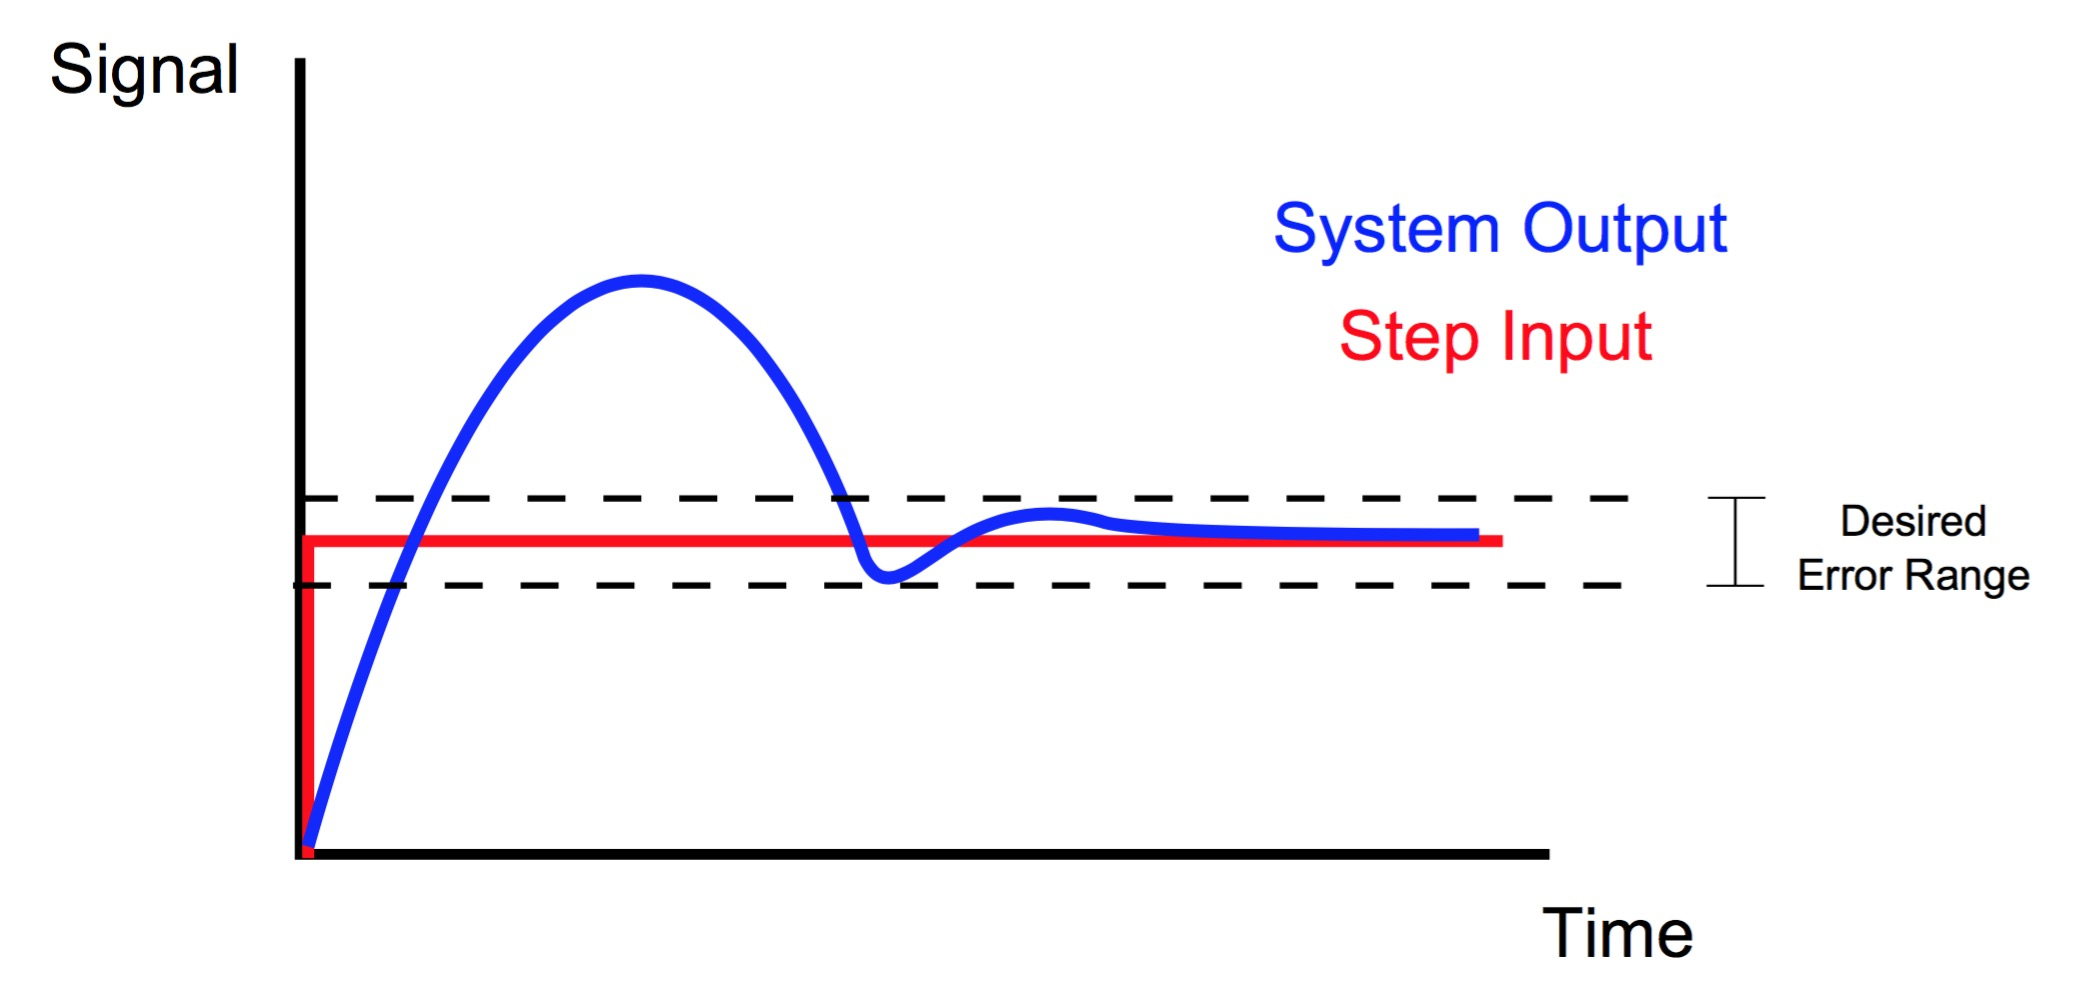
\includegraphics[width=4.5in]{stable_system.jpg} 
   \caption{Example of a Stable System}
   \label{fig:example}
\end{figure}


\newpage

\section*{\fontsize{12}{12}\selectfont \large Procedure \& Analysis}
\addcontentsline{toc}{section}{Procedure \& Analysis} % Add for each section
First, the signal flow graph was sketched using the Phase Variable Method and the state-space equations were written, as shown in Figure 2. The system was then analyzed in MATLAB to obtain the state-space equations, shown in Figure 3, and the results were compared to the equations found by hand in Figure 2. The step response of the system was then obtained, and is shown in Figure 3 along with the response information shown in Figure 4. As seen in Figure 3, the system tends to oscillate around a central value with increasing amplitude; therefore, the system does not approach any constant value as times goes on and is therefore unstable. Figure 4 also shows that the system is unstable because the peak and peak time are infinity, yielding no definitive overshoot, rise time, settling time, or settling value.
\bigskip

The system was then modeled in Simulink, as shown in Figure 5. The step response was obtained from the model and is shown in Figure 6. Note that the only difference between the responses in Figure 3 and Figure 6 is that the step input is not initiated at the same time. 
\bigskip
\bigskip

% Figures here

\begin{figure}[htbp] %  figure placement: here, top, bottom, or page
   \centering
   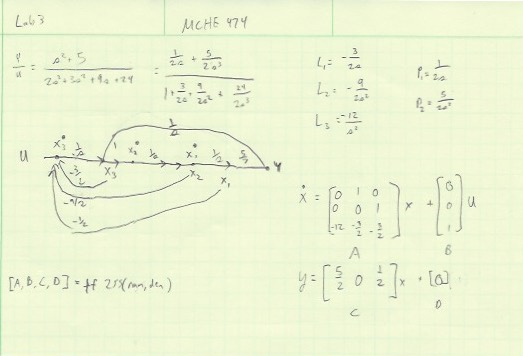
\includegraphics[width=\linewidth]{handwritten_calculations.jpeg} 
   \caption{State-Space Equations by Hand}
   \label{fig:example}
\end{figure}

\newpage

\begin{figure}[h!] %  figure placement: here, top, bottom, or page
   \centering
   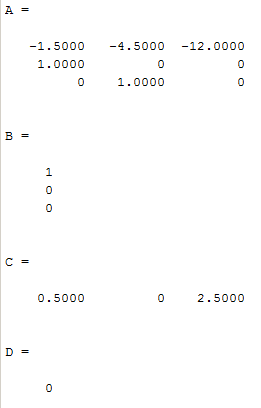
\includegraphics[width=2in]{coefficient_matrices.PNG} 
   \caption{State-Space Equations using MATLAB}
   \label{fig:example}
\end{figure}

\bigskip

\begin{figure}[h!] %  figure placement: here, top, bottom, or page
   \centering
   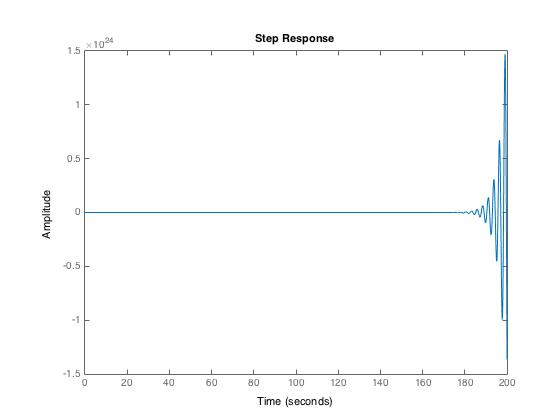
\includegraphics[width=6in]{matlab_script_time_response.jpg} 
   \caption{System Time Response (MATLAB)}
   \label{fig:example}
\end{figure}

\newpage

\bigskip
\bigskip
\begin{figure}[h!] %  figure placement: here, top, bottom, or page
   \centering
   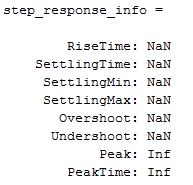
\includegraphics[width=2.5in]{step_response_info.PNG} 
   \caption{System Step Response Information}
   \label{fig:example}
\end{figure}

\bigskip
\bigskip

\begin{figure}[h!] %  figure placement: here, top, bottom, or page
   \centering
   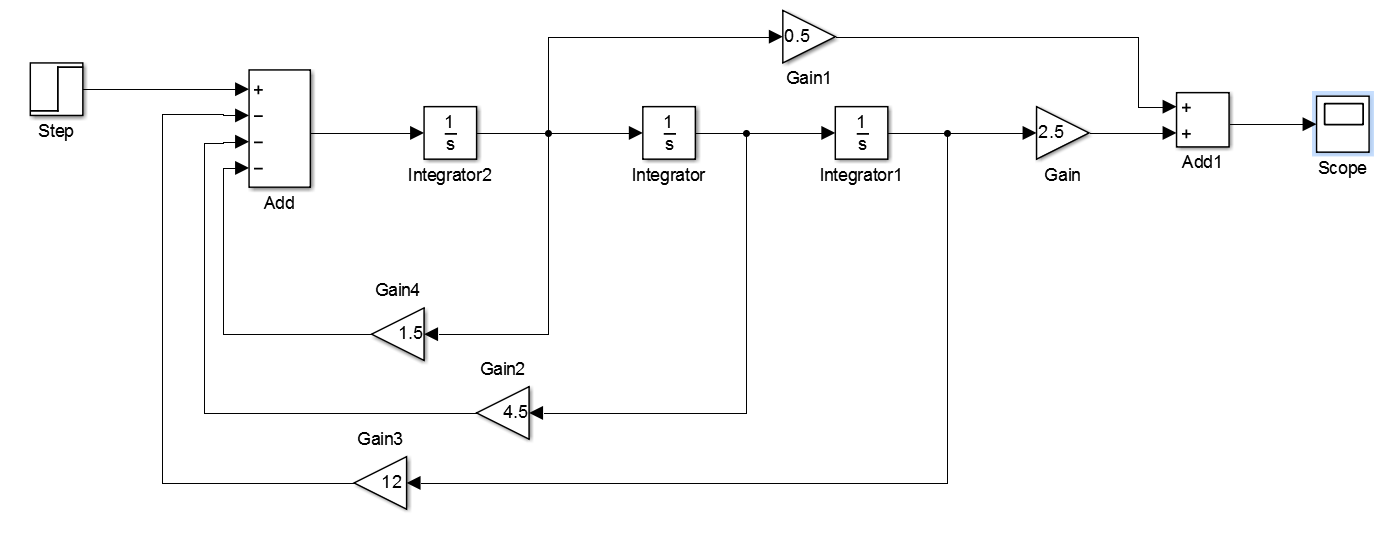
\includegraphics[width=\linewidth]{simulink_model_pic.PNG} 
   \caption{Simulink Model}
   \label{fig:example}
\end{figure}

\newpage

\begin{figure}[htbp] %  figure placement: here, top, bottom, or page
   \centering
   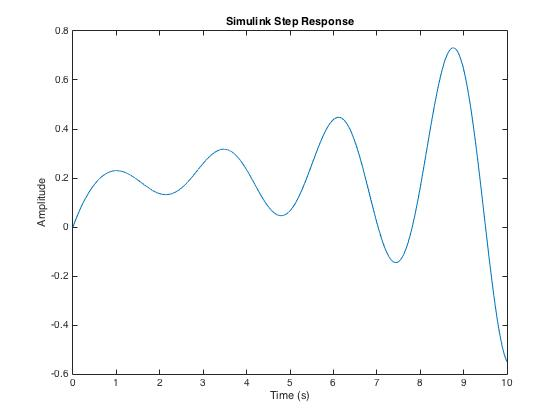
\includegraphics[width=6in]{simulink_model_time_response.jpg} 
   \caption{System Time Response (Simulink)}
   \label{fig:example}
\end{figure}

\bigskip


\section*{\fontsize{12}{12}\selectfont \large Conclusion}
\addcontentsline{toc}{section}{Conclusion} % Add for each section
The exercises conducted in this lab reinforce the theory learned in the classroom. It is shown that systems can be analyzed in the time domain, which is better than analyzing a system in the frequency domain for complex systems. Obtaining the state-space equations and modeling of a system is very important in the field of controls; therefore, this experience with state-space representations of linear control system is very beneficial.




%\section*{\fontsize{12}{12}\selectfont \large References}

\begin{thebibliography}{2}

% Example
%\bibitem{Wagner}
%Ng, K., Wagner, S.W., Camelio, J., Emblom, W.J. (2010). ?Experimental Analysis of Micro Tube
%Hydroforming Process.? Transactions of NAMRC of SME, 38, 577-584.

\end{thebibliography}



%\section*{\fontsize{12}{12}\selectfont APPENDIX}

%\begin{table}[h!]
%  \caption{}
%  \includegraphics[width=\linewidth]{table1.png}
%\end{table}




\end{document}







----------------------------Templates-------------------------------

-------------------------Figure-----------------------

\begin{figure}[h!]  
  \centering
    \includegraphics[width=\linewidth]{**file**}
    \caption{Docking Station}
\end{figure}

---------------------------Table-----------------------
\begin{table}[ht]
\caption{Nonlinear Model Results} % title of Table
\centering % used for centering table
\begin{tabular}{c c c c} % centered columns (4 columns)
\hline\hline %inserts double horizontal lines
Case & Method\#1 & Method\#2 & Method\#3 \\ [0.5ex] % inserts table
%heading
\hline % inserts single horizontal line
1 & 50 & 837 & 970 \\ % inserting body of the table
2 & 47 & 877 & 230 \\
3 & 31 & 25 & 415 \\
4 & 35 & 144 & 2356 \\
5 & 45 & 300 & 556 \\ [1ex] % [1ex] adds vertical space
\hline %inserts single line
\end{tabular}
\label{table:nonlin} % is used to refer this table in the text
\end{table}



probably best to insert as an image from excel

\bigskip\\
\begin{table}[h!]
  \caption{}
  \includegraphics[width=\linewidth]{**file**}
\end{table}
\bigskip\\





-----------------------------Equations------------------------
-----------------------------Regular
\begin{equation}
a = b + c
\end{equation}

--------------------------------- Multiline
\begin{multline}
a = b + c + d + e + f
+ g + h + i + j \\
+ k + l + m + n + o
\end{multline}

-------------------------------Citations-------------------------
\bibitem{Author last name}
  Last, First., year of publication,
  article name, book(etc) name, from \\
  link goes here

----------------------------------other-----------------------------

equations:
http://moser-isi.ethz.ch/docs/typeset_equations.pdf

citations:
http://library.missouri.edu/engineering/about/guides/asme
https://www.asme.org/shop/proceedings/conference-publications/references